%Dokumentenklasse "scrbook" - Erweitert um den Verweis auf die Verzeichnisse und Texteigenschaften
\documentclass[chapterprefix=true, 12pt, a4paper, oneside, parskip=half, listof=totoc, bibliography=totoc, numbers=noendperiod]{scrbook}

% Ränder (Standard bottom ca. 52mm anbzüglich von ca. 4mm für die nach oben rechts gewanderte Seitenzahl)
%Anpassung der Seitenränder
\usepackage[bottom=32mm,left=25mm,right=25mm]{geometry}

% Ränder bei Bedarf zeigen
%\usepackage{showframe}

%Tweaks für scrbook
\usepackage{scrhack}

%Blindtext
\usepackage{blindtext}

%Erlaubt unteranderem Umbrücke captions
\usepackage{caption}

%Stichwortverzeichnis
\usepackage{imakeidx}

%Kompakte Listen
\usepackage{paralist}

%Zitate besser formatieren und darstellen
\usepackage{epigraph}

%Glossar + Stichworverzeichnis
\usepackage[toc, acronym]{glossaries} % Akronyme werden als eigene Liste aufgeführt
\glsenablehyper

%Anpassung von Kopf- und Fußzeile
%beinflusst die erste Seite des Kapitels
\usepackage[automark,headsepline]{scrlayer-scrpage}
\automark{chapter}
\ihead{\leftmark}
\chead{}
\ohead{\thepage}
\ifoot*{}
\cfoot[\thepage]{}
\cfoot*{}
\ofoot*{}
\pagestyle{scrheadings}

%Auskommentieren für die Verkleinerung des vertikalen Abstandes eines neuen Kapitels
%\renewcommand*{\chapterheadstartvskip}{\vspace*{.25\baselineskip}}

%Zeilenabstand 1,5
\usepackage[onehalfspacing]{setspace}

%Verbesserte Darstellung der Buchstaben zueinander
\usepackage[stretch=10]{microtype}

%Deutsche Bezeichnungen für angezeigte Namen (z.B. Innhaltsverzeichnis etc.)
\usepackage[ngerman]{babel}

%Unterstützung von Umlauten und anderen Sonderzeichen (UTF-8)
\usepackage{lmodern}
\usepackage[utf8]{luainputenc}
\usepackage[T1]{fontenc}

%Einfachere Zitate
\usepackage{epigraph}

%Verwendung von Akronymen
\usepackage[printonlyused]{acronym}

%Unterstützung der H positionierung (keine automatische Verschiebung eingefügter Elemente)
\usepackage{float} 

%Erlaubt Umbrüche innerhalb von Tabellen
\usepackage{tabularx}

%Erlaubt Seitenumbrüche mit Tabellen
\usepackage{longtable}

%Erlaubt die Darstellung von Sourcecode mit Highlighting
\usepackage{listings}

%Definierung eigener Farben bei nutzung eines selbst vergebene Namens
\usepackage[table,xcdraw]{xcolor}

%Vektorgrafiken tikz
\usepackage{tikz}

%Grafiken (wie jpg, png, etc.)
\usepackage{graphicx}

%Grafiken von Text umlaufen lassen
\usepackage{wrapfig}

%Grafik bestehend aus mehreren Grafiken
\usepackage{subfigure}

%Ermöglicht Verknüpfungen innerhalb des Dokumentes (e.g. for PDF), Links werden durch "hidelink" nicht explizit hervorgehoben
\usepackage[hidelinks,ngerman]{hyperref}

%Einbindung und Verwaltung von Literaturverzeichnissen
\usepackage{csquotes} %wird von biber benötigt
\usepackage[style=alphabetic, backend=biber, bibencoding=utf8]{biblatex}
\addbibresource{references/references.bib}

%enable the macro \mathbb
\usepackage{amssymb}
\usepackage{amsmath}

%-------------------------------Zusätzliche Anpassungen und Modifikationen--------------------------------------------%

%Anpassung der Überschriften
\addtokomafont{disposition}{\rmfamily}

%Zusätzliche Farben
\definecolor{Ao}{rgb}{0.0, 0.39, 0.0}
\definecolor{antiquefuchsia}{rgb}{0.57, 0.36, 0.51}
\definecolor{bostonuniversityred}{rgb}{0.8, 0.0, 0.0}

% Padding für images innerhalb von longtables
\usepackage{verbatimbox}
\newcommand\Includegraphics[2][]{\addvbuffer[5pt 0pt]{\includegraphics[#1]{#2}}}

%Umbenennungen
\renewcommand{\lstlistlistingname}{Source Code Content}

%Pluszeichen in der Reference beim zitieren ausblenden
\renewcommand*{\labelalphaothers}{}

%Anpassugen zur Quelltextdarstellung, kann bei Bedarf überschrieben werden (z.B. wenn unterschiedliche Sprachen zum Einsatz kommen)
\renewcommand{\lstlistingname}{Code snippet}
\lstset{
	language=python,
	numbers=left,
	columns=fullflexible,
	aboveskip=5pt,
	belowskip=10pt,
	basicstyle=\small\ttfamily,
	backgroundcolor=\color{black!5},
	commentstyle=\color{black},
	morecomment=[s]{.s}{hape}, % workaround to exclude ".shape"
	keywordstyle=\color{antiquefuchsia},
	otherkeywords={self, else},
	emphstyle=\color{bostonuniversityred},
	emph={shape,units,name,filters,kernel_size,activation,padding,kernel_initializer,kernel_regularizer,bias_initializer,inputs,outputs,mode,distribution,minval,maxval, callback_args, low, high, limit, window_length, size, mu, theta, sigma},
	stringstyle=\color{Ao},
	showspaces=false,
	showstringspaces=false,
	showtabs=false,
	xleftmargin=16pt,
	xrightmargin=0pt,
	framesep=5pt,
	framerule=1pt,
	frame=leftline,
	rulecolor=\color{black},
	tabsize=2,
	breaklines=true,
	breakatwhitespace=true
}

%Anpassungen für das Abkürzungsverzeichnis
\newglossarystyle{dottedlocations}{%
	\glossarystyle{list}%
	\renewcommand*{\glossaryentryfield}[5]{%
		\item[\glsentryitem{##1}\glstarget{##1}{##2}] \emph{##3}%
		\unskip\leaders\hbox to 2.9mm{\hss.}\hfill##5}%
	\renewcommand*{\glsgroupskip}{}%
}

% Titles Config - CHOOSE ONE section for title format

%% Used for titleGraduation Bachelor
%% Based on https://ai-bachelor.htw-berlin.de/files/Stg/AI/richtlinie_ba-arbeit_ai_06_02_13.pdf
\makeatletter

\newcommand*{\gradeType}[1]{\gdef\@gradeType{#1}}
\newcommand*{\firstExaminer}[1]{\gdef\@firstExaminer{#1}}
\newcommand*{\secondExaminer}[1]{\gdef\@secondExaminer{#1}}
\newcommand*{\matrikelnr}[1]{\gdef\@matrikelnr{#1}}
\newcommand*{\submitDate}[1]{\gdef\@submitDate{#1}}

\renewcommand*{\maketitle}{
	\begin{titlepage}
		\newgeometry{left=2.5cm,right=2.5cm,top=2.5cm,bottom=2.5cm}
		\begin{figure}[H]
			\centering
			
\includegraphics[width=0.5\textwidth]{resources/htw/logo}
		\end{figure}
		\begin{center}
			\vfill
			{\Large \@title\par}
			\vskip 0.5cm
			{\large \bfseries Projektarbeit\par}
			\vskip 0.5cm
			{\large an der}
			\vskip 0.5cm
			{\large Hochschule für Technik und Wirtschaft Berlin}
			\vskip 0.0cm
			{\large Kurs Mobile Anwendungen}
			\vskip 0.0cm
			{\large Studiengang Angewandte Informatik}
			\vfill
			\begin{flushleft}
				\begin{tabular}[t]{rl}
					Betreuer: &\@firstExaminer\\
					\\
					Eingereicht von: &\@author\\
					Immatrikulationsnummer: & \@matrikelnr\\
					Eingereicht am: & \@submitDate
				\end{tabular}
			\end{flushleft}
		\end{center}
		\restoregeometry
	\end{titlepage}
}
\makeatother
\gradeType{Bachelor of Science (B.Sc.)}

%% Used for titleGraduation Master
%% Based on https://ai-master.htw-berlin.de/files/Stg/AI/richtlinie_ma-arbeit_ai_25_01_13.pdf
%\makeatletter

\newcommand*{\gradeType}[1]{\gdef\@gradeType{#1}}
\newcommand*{\firstExaminer}[1]{\gdef\@firstExaminer{#1}}
\newcommand*{\secondExaminer}[1]{\gdef\@secondExaminer{#1}}
\newcommand*{\matrikelnr}[1]{\gdef\@matrikelnr{#1}}
\newcommand*{\submitDate}[1]{\gdef\@submitDate{#1}}

\renewcommand*{\maketitle}{
	\begin{titlepage}
		\newgeometry{left=2.5cm,right=2.5cm,top=2.5cm,bottom=2.5cm}
		\begin{figure}[H]
			\centering
			
\includegraphics[width=0.5\textwidth]{resources/htw/logo}
		\end{figure}
		\begin{center}
			\vfill
			{\Large \@title\par}
			\vskip 0.5cm
			{\large \bfseries Projektarbeit\par}
			\vskip 0.5cm
			{\large an der}
			\vskip 0.5cm
			{\large Hochschule für Technik und Wirtschaft Berlin}
			\vskip 0.0cm
			{\large Kurs Mobile Anwendungen}
			\vskip 0.0cm
			{\large Studiengang Angewandte Informatik}
			\vfill
			\begin{flushleft}
				\begin{tabular}[t]{rl}
					Betreuer: &\@firstExaminer\\
					\\
					Eingereicht von: &\@author\\
					Immatrikulationsnummer: & \@matrikelnr\\
					Eingereicht am: & \@submitDate
				\end{tabular}
			\end{flushleft}
		\end{center}
		\restoregeometry
	\end{titlepage}
}
\makeatother
%\gradeType{Master of Science (M.Sc.)}
%\secondExaminer{TODO}

%% Used for titleResearchProject
%% Based on http://christianherta.de/lehre/HTW/richtlinie-wissenschaftliche-Arbeiten.pdf
%\makeatletter

\newcommand*{\firstExaminer}[1]{\gdef\@firstExaminer{#1}}
\newcommand*{\subTitle}[1]{\gdef\@subTitle{#1}}
\newcommand*{\researchPart}[1]{\gdef\@researchPart{#1}}
\newcommand*{\matrikelnr}[1]{\gdef\@matrikelnr{#1}}
\newcommand*{\submitDate}[1]{\gdef\@submitDate{#1}}


\renewcommand*{\maketitle}{
	\begin{titlepage}
		\newgeometry{left=2.5cm,right=2.5cm,top=2.5cm,bottom=2.5cm}
		\begin{figure}[H]
			\centering
			
\includegraphics[width=0.5\textwidth]{resources/htw/logo}
		\end{figure}
		\begin{center}
			\vfill
			{\Large \@title\par}
			\vskip 0.5cm
			{\large \bfseries Forschungsprojekt \@researchPart\par}
			\vskip 0.5cm
			{\large an der}
			\vskip 0.5cm
			{\large Hochschule für Technik und Wirtschaft Berlin}
			\vskip 0.0cm
			{\large Fachbereich Wirtschaftswissenschaften II}
			\vskip 0.0cm
			{\large Studiengang Angewandte Informatik}
			\vfill
			\begin{flushleft}
				\begin{tabular}[t]{rl}
					Supervisor: &\@firstExaminer\\
					\\
					Submitted by: &\@author\\
					Matriculation Number: & \@matrikelnr\\
					Submission Date: & \@submitDate
				\end{tabular}
			\end{flushleft}
		\end{center}
		\restoregeometry
	\end{titlepage}
}
\makeatother
%\researchPart{A/B} % choose A or B

% Titles Config End

% Used by all titles
\title{Konzeption und Realisierung eines automatisierten künstlichen Sonnenlichts}
\author{Leon Enzenberger}
\matrikelnr{s0568823}
\submitDate{26.03.2021}
\firstExaminer{Prof. Dr. A. Huhn}
% End Titles

\makeindex[title=Index, options=-s indexstyle.ist, intoc]
\indexsetup{level=\chapter*,toclevel=chapter}

\loadglsentries{glossary_and_acronyms.tex}
\setacronymstyle{long-short}
\begin{document}

\pagenumbering{alph} % fix for same identifier warning, character is not show in title
\maketitle

\pagenumbering{roman}
\chapter*{Vorwort}

Die vorliegende Projektarbeit entstand im Rahmen meines Studiums der Angewandten Informatik an der Hochschule für Technik und Wirtschaft Berlin.

Die Idee zu diesem Projekt entstand am Anfang der Wintermonate, als das Tageslicht immer weniger wurde. Wie vermutlich bei vielen weiteren Menschen, fällt bei mir die Stimmung, und damit auch die Produktivität, bei zu wenig Tageslicht ab. Um gegen diesen Umstand vorzugehen, suchte ich nach Lösungen für dieses Problem. Dabei stieß ich auf ein Design einer Beleuchtung, die nicht nur die Farbtemperatur von Sonnenlicht, sondern auch die Parallelität der Strahlen, die diffuse Streuchcharakteristiken und sogar ansatzweise die Intensität nachahmt. Eine der Kernkomponenten dieser Lampe ist ein 100w-500w starke LED.

Schon vor Beginn des Nachbaus dieser Idee, kamen mir einige Bedenken. Zum einem verbraucht eine solche Beleuchtung ein vielfaches des Stroms konventioneller und zeitgemäßer Leuchtmittel. Zum anderen sah ich die Gefahr durch die Beleuchtung meinen Tagesrhythmus unbeabsichtigt aus dem Rhythmus zu bringen.

Um sicherzustellen, dass diese Beleuchtung nur an ist, wenn sie aufgrund mangelndem natürlichem Lichts benötigt wird und sie außerdem den Nutzer nicht aus versehen bis tief in die Nacht wach hält, bot sich eine Automatisierung der Schaltung an. Diese Arbeit soll den Prozess der Realisierung der Hard- sowie Software darstellen.

Mein Dank gilt Prof. Dr. Huhn für die Beratung zur Wahl der elektronischen Komponenten sowie der Software-Plattform und meiner Freundin Juliya Rajasingam für die Hilfe bei der Beschaffung aller nicht elektronischen Komponenten und als (mehr oder weniger) freiwilliges Testsubjekt.

Ich hoffe allen Lesern gut die Erfahrungen vermitteln zu können, die ich bei der Durchführung dieses Projektes gesammelt habe.


Leon Enzenberger

Berlin, 24.06.2020
 \clearpage  % FOR BA/MA-THESIS, NOT REQUIRED FOR RESEARCHPROJECT
\chapter*{Kurzbeschreibung}
Die Wintermonate schlagen bei vielen Menschen durch mangelnde Sonnenstrahlung auf die Stimmung. Um diesem Effekt entgegen zu wirken gibt es sogenannte \glqq Sonnenlichtlampen\grqq{}. Diese simulieren jedoch nur ausgewählte Aspekte echter Sonnenstrahlen. Die Projektarbeit erläutert einen erweiterten technologischen Ansatz der Beleuchtung, der jedoch verhältnismäßig viel Energie verwendet und versucht ihn mithilfe geeigneter IOT-Technik effizienter zu gestalten, die Bedienung für den Nutzer via eines Smartphones zu ermöglichen und die Beleuchtung mithilfe von Automatisierung in den Hintergrund verschwinden zu lassen. \clearpage

\tableofcontents \newpage

\pagenumbering{arabic}
\chapter{Einleitung}


\section{Motivation}
Sonnenlicht ist die wohl bedeutendste Energiequelle für uns Menschen. Durch Photosynthese gedeihen Pflanzen und bilden damit den Anfang der Nahrungskette. Wir gewinnen Strom durch Solarzellen, Wind- und Wasserkraftwerke, welche direkt oder indirekt durch Sonnenstrahlen ermöglicht werden.

Sonnenstrahlen spielen jedoch auch für unseres mentale Verfassung eine wichtige Rolle. Ohne sie kann der menschliche Körper kein Vitamin D-Erzeugen, was gesundheitliche Komplikationen mit sich ziehen kann. Zudem kann das Fehlen auf die Stimmung und die Motivation schlagen.

Gerade in den Wintermonaten können die kürzeren und schwächeren Sonnenperioden bei Menschen eine sogenannte \glqq Winterdepression\grqq{} verursachen \cite{Ban20}, die sich auf das persönliche wie professionelle Leben auswirken kann. Folglich ist es für jeden Betroffenen wünschenswert einem Lichtmangel entgegenzuwirken.

Das ausbleiben der Körpereigenen Vitamin-D Produktion kann durch die Einnahme von Nahrungsergänzungsmitteln ausgeglichen werden. Doch die ermunternde Wirkung von Tageslicht besitzen diese Mittel leider nicht.

\section{Zielsetzung}
Mit dem Aufkommen von LEDs, die das Strahlungsspektrum des sichtbaren Lichtes überzeugend simulieren können, haben sich sogenannte Tageslichtlampen auf dem Markt etabliert. Diese simulieren aber nur wenige Charakteristiken von echtem Sonnenlicht. Diese Arbeit soll die Idee eines Youtubers für ein Design einer Lampe mit realistischeren Charakteristika aufgreifen und in ein paar Aspekten verbessern.

Eine Eigenschaft der Beleuchtung mit Optimierungspotential ist die Stromaufnahme. Denn das Design der Lampe nutzt, je nach Konfiguration, eine 100w bis 500w starke LED. Diese ermöglicht eine realistisch helle Beleuchtung, hat aber eine entsprechend hohe Leistungsaufnahme. Um diese zu verbessern, sollte das Licht nur eingeschaltet sein, wenn nicht genügend natürliches Tageslicht zur Verfügung steht. 

Zudem sollte das Licht je nach Tageszeit an oder aus gehen, um nur in Wachspanne des Nutzers eingeschaltet zu sein. Eine solche Zeit-schalt-Funktion kann zudem dafür genutzt werden, den Nutzer zur richtigen Zeit mit \glqq Sonnenstrahlen\grqq{} zu wecken, oder daran erinnern, zeitnah ins Bett zu gehen.

\section{Vorgehensweise und Aufbau der Arbeit}

Der Aufbau dieser Arbeit ist im Folgenden beschrieben. Zunächst werden die physikalischen Grundlagen einer solchen Beleuchtungseinrichtung dargelegt. Danach wird erläutert, wie die genutzte Hardware- und Softwareplattformen gewählt wurden und ihre grundlegende Eignung für diesen Aufgabenbereich festgestellt wurde. Darauf aufbauend wird die Konzeption der Kommunikation zwischen den einzelnen Komponenten und die Gestaltung des User-Interfaces veranschaulicht. Im Anschluss wird die Implementierung und das Testvorgehen behandelt. Zuletzt wird das abschließende Ergebnis bewertet und ein Fazit aus dem resultierenden Ergebnissen gezogen.


 \clearpage
\chapter{Pysikalische Grundlagen}

Sonnenlicht hat auf der Erdoberfläche einige besondere Charakteristiken, die sich im Laufe des Tages auch verändern können. Dazu zählen unter anderem:

\begin{compactitem}
	\item Farbtemperatur
	\item Aufteilung in diffusen und direkten Anteil
	\item Einfallswinkel
	\item Parallelität der Strahlen
	\item Intensität
\end{compactitem}

Die \textbf{Farbtemperatur} des Sonnenlichtes kommt von der spezifischen chemischen Zusammensetzung der verschiedenen strahlenden Elemente. 

Wenn sich dieses Licht durch die Atmosphäre der Erde bewegt, werden die kurzwelligen Strahlen durch Partikel und Moleküle einfacher abgelenkt als Langwellige. So erscheint die Sonne mittags gelb (langwelligere Strahlen), im Gegensatz zum blauen Himmel (kurzwelligere Strahlen), der durch das abgelenkte Licht erleuchtet ist. Diese Aufteilung führt zu einer \textbf{diffus} blauen und einer \textbf{direkten} gelben Beleuchtung.

Durch die Drehung der Erde verändert sich der \textbf{Einfallswinkel} der Sonnenstrahlen jedoch. So müssen sie morgens und abends mehr Atmosphäre durchdringen als Mittags. Hierdurch kann noch mehr Licht gefiltert werden, wodurch sich die \textbf{Farbtemperatur} und \textbf{Intensität} des Lichtes stark ändern kann. Den farblichen Unterschied kann mit Kelvin gemessen werden, die Intensität mit Lux.

Die nahezu \textbf{parallele Orientierung der Lichtstrahlen} kommt von der weiten Entfernung der Sonne zur Erde. Der Effekt ist, dass ein Objekt immer einen gleich großen Schatten wirft, egal wie weit es von der Lichtquelle entfernt ist.
 \clearpage
\chapter{Analyse}

\section{Hardware Analyse}

Für die vollständige Umsetzung der im letzten Abschnitt genannten Aspekte in einem Leuchtmittel sind die folgenden Hauptkomponenten nötig:

\begin{compactitem}
	\item Leuchtmittel mit genügend Ausgangsleistung
	\item Möglichkeit zum dimmen des Leuchtmittels
	\item Komponente zur Steuerung der Streucharakteristik des Lichts
	\item Komponente zur Erreichung einer realistischen Diffusion des Lichts
	\item Aufhängung, die ein automatisiertes Schwenken erlaubt
	\item Möglichkeit der Steuerung und Automatisierung der Beleuchtung
\end{compactitem}


\section{Funktionale Anforderungen}
Damit die Beleuchtung den Nutzer effektiv unterstützen kann, bedarf es einer Bedienoberfläche, mit der das gewünschte Verhalten der Lampe eingestellt werden kann. Da dieses Verhalten vom Nutzer abhängig ist und ihn bei seiner Tagesplanung unterstützen sollte, müssen mindestens die folgenden Parameter einstellbar und einsehbar sein:

\begin{compactitem}
	\item Automatische Ein- und Ausschaltzeit der Beleuchtung
	\item Schwellenwert, bei dem das Licht die Rolle der Sonne übernimmt
	\item Wechsel zwischen manuellem und autonomen Modus um das Licht wie eine reguläre Lampe verwenden zu können
\end{compactitem}

\section{Nichtfunktionale Anforderungen}
Die Nutzung der autonomen Funktion ist gerade für dieses Projekt Kernbereich der Arbeit. Im Idealfall sollte die Lampe nur ein einziges Mal eingestellt werden und danach vollkommen autonom ein- und ausschalten. Aus diesem Grund ist ein hohes Maß an Zuverlässigkeit für diese Funktion von Nöten. Des weiteren sollte das Nutzer-Interface möglichst intuitiv zu bedienen sein und die einzelnen Funktionen so wenig Interaktion wie möglich verlangen. Damit soll die reibungslose Nutzung sichergestellt werden und durch das Vertrauen auf den Autonomen Betrieb Energie gespart werden. \clearpage
\chapter{Konzeption}

\section{Vorangehende Arbeit}
Diese Arbeit baut auf dem Design des Youtubers \glqq Matthew Perks\grqq{} auf. Sein Ziel war es eine Beleuchtung zu schaffe, die in den dunklen Monaten die Stimmung hebt und damit die Produktivität des Nutzers fördert \cite{Perks20}. Vermutlich aus Kosten und Komplexitätsgründen wurde auf die Variabilität der Farbtemperatur und den veränderlichen Einfallswinkel verzichtet.

Als Lichtquelle nutzt dieses Design eine COB-LED mit 500w Leistung, einem hohen CSI-Index von 95 und einem Kelvinwert von 5600, was die Beleuchtung durch Morgensonne realistisch nachahmt. Zur Kühlung dieser Led wird eine System auf Basis einer Wasserkühlung für einen Computer verwendet. Um die Lichtstrahlen der LED parallel auszurichten, baute er mithilfe von reflektierender Folie eine Satellitenschüssel zu einem Parabolspiegel um. Die letzte ausschlaggebende Komponente ist ein dünnes, einem Fenster ähnliches transparentes Behältnis das mit Seifenwasser befüllt ist. Dies dient zur Simulation der Atmosphäre, da hier das Licht durch die kleinen Partikel ebenso in einen diffusen bläulichen und einen direkten gelblich Anteil aufgespalten wird.

\begin{figure}[H]
	\centering
	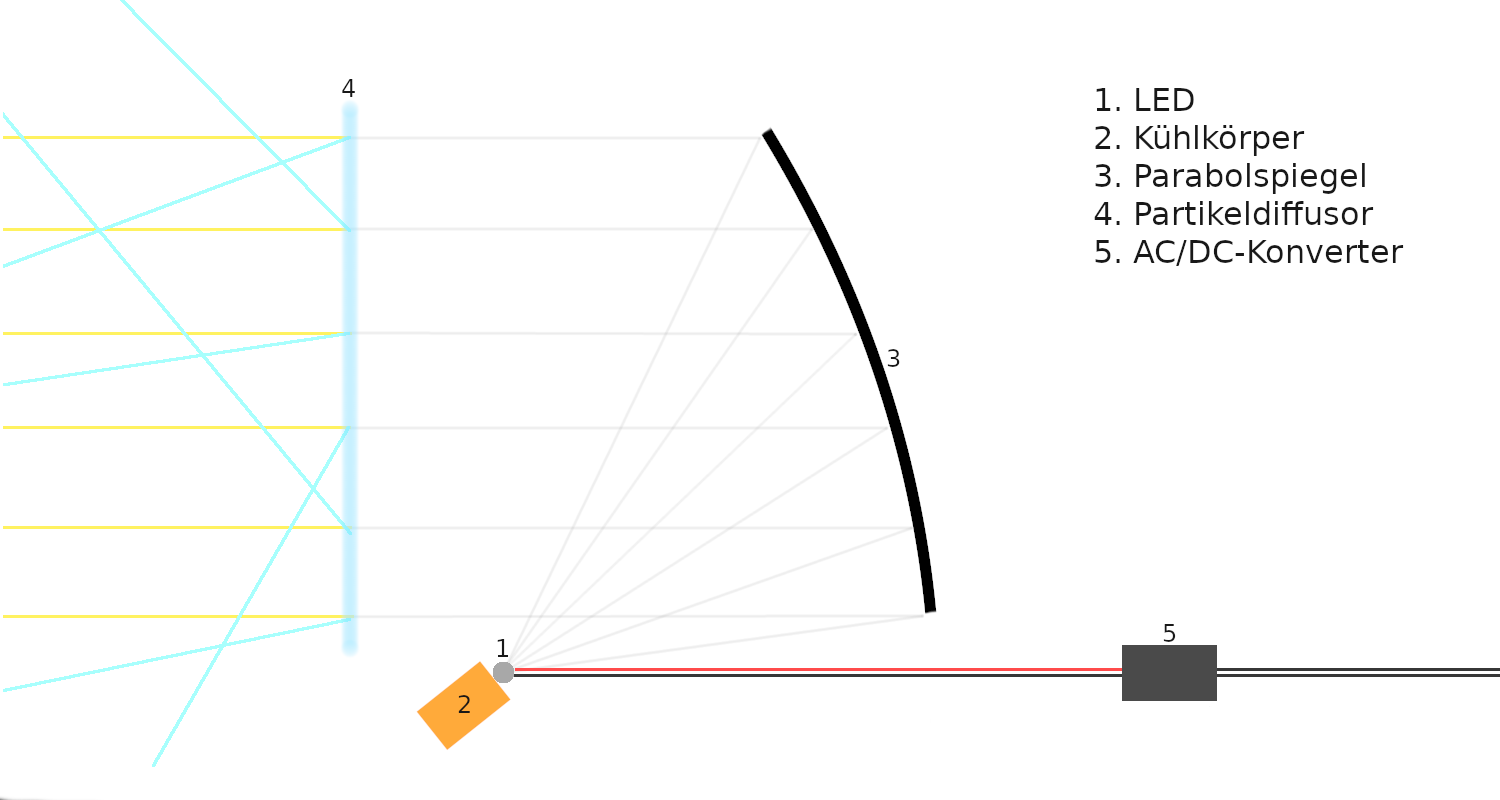
\includegraphics[width=0.95\textwidth]{resources/own_content/sun-design}
	\caption{Funktionsprinzip der Beleuchtung \cite{LePr}}
	\label{img:funktions_prinzip}
\end{figure}

\section{Hardware Konzeption}
Das Design braucht noch einige elektronische Komponenten um automatisiert betrieben zu werden. So braucht es zumindest einen Mikrocontroller um Daten verarbeiten zu können. Dieser Mikrocontroller braucht zudem einen Lichtsensor um auf die Beleuchtungssituation reagieren zu können. Zudem braucht es einen Weg, die Einstellungen einzusehen und manipulieren zu können. 

Da Mikrocontroller in der Regel nicht direkt mit der hohen benötigten Leistung der LED arbeiten können, wurde eine Schnittstelle zwischen Mikrocontroller und der Stromzufuhr der LED benötigt. Aus Gründen der Komplexität wird hier ein Relais vorgesehen. Ein Dimmer würde einen fließenden Übergang zwischen natürlichem um künstlichem Licht ermöglichen. Doch aufgrund mangelnder elektrotechnischer Erfahrung wird in dieser Arbeit auf die einfachere Art der binären Schaltung gesetzt.

Abschließend brauchen diese beiden weiteren Komponenten auch eine Stromversorgung. Zwar nutzt das grundlegende Design schon ein Leistungsfähiges Netzteil, dieses kann aber wegen der unpassenden Spannung nicht direkt für den Mikrocontroller und das Relais genutzt werden. Denn im Gegensatz zu der LED nutzen diese Komponente in der Regel eine sehr viel niedrigere Arbeitsspannung. Aus diesem Grund ist mindestens ein Buck-Konverter für die Wandlung des Stroms von Nöten. Hierdurch können alle Komponenten durch ein einzige Stromquelle versorgt werden.

\section{Software Konzeption}

\subsection{Grundlegende Architekturen}
Da ein Mikrocontroller in der Regel nicht mit Hardware zur Anzeige oder Intuitiven Eingabemöglichkeiten ausgestattet ist, muss diese anderweitig bereit gestellt werden. Glücklicherweise erfreuen sich Smartphones weiter Verbreitung und stellen mit ihren Displays ideale Kandidaten für das Interface dieses Anwendungszweck dar. Aufgrund des hohen Marktanteils wurde Android als Zielplattform gewählt.

Die Wahl der Software für den Mikrocontroller viel auf Micropython. Diese Wahl wurde aufgrund des Hohen Abstraktionsgrades dieser Sprache gewählt, wodurch eine potentiell schnelle Implementierung der Funktionen ermöglicht werden sollte.

\subsection{Kommunikation der Komponenten}
Die Kommunikation zwischen diesen beiden Plattformen sollte drahtlos per TCP über Wifi passieren. Diese Wahl wurde unter der Annahme getroffen, das eine solche Lampe nur stationär in der Wohnung des Besitzer verwendet wird, wo schon ein Wlan aufgespannt wurde. Im Gegensatz zu Bluetooth hat dies den Vorteil, dass nicht jedes mal erst ein Pairing-Prozess angestoßen werden muss um die Beleuchtung anpassen zu können und davon ausgegangen werden kann, dass zuhause mobile Endgeräte sowieso schon hiermit verbunden sind.

\subsection{Nutzerinterface}
Damit die Lampe möglichst intuitiv zu bedienen ist und alle Funktionen nicht mehr als einen Klick benötigen, sollten alle Features von einem zusammenhängendem Panel erreichbar sein. Zudem sollten die meist genutzten Funktionen in der Nähe des Daumens verortet sein, um sie noch einfacher erreichbar zu machen. Es kann davon ausgegangen werden, dass ein durchschnittlicher Mensch nicht mit Einheiten zur Messung der Lichtintensität und schon gar nicht mit ihrer Interpretation vertraut ist. Aus diesem Grund wurde die Visualisierung der Messdaten des Vortages in Form von Graphen eingeplant, um dem Nutzer einen Orientierungspunkt für Konfigurationen zu bieten. Dieser sollte die Zeit in der x-Achse und die Lichtintensität an der y-Achse widerspiegeln. Dies legte die Wahl nahe, Schieberegler an den beiden Achsen zu platzieren um eine intuitive Einstellung der Zeit- und Lichtschwellenwerte für die Ein- und Ausschaltzeitpunkte zu ermöglichen. Zudem sollten alle momentanen Einstellungen in der Applikation ersichtliche sein. Dies soll durch eine entsprechende Farbgebung der Buttons und der entsprechenden Platzierung der Schieberegler möglich sein. Um eine Verbindung aufzubauen, muss ebenfalls eine Eingabe möglich sein. Da im vorherigen Abschnitt die Wahl der Kommunikation auf TCP fiel, sollte hier die IP-Adresse eingegeben werden. Da sich die IP wegen dem stationären Einsatzgebiets der Lampe nur, selten ändern sollte, wurde dieses Eingabefeld mit niedriger Priorität an den Oberen Rand des Panels geschoben. Das resultierende Design ist in der folgenden Abbildung ersichtlich.

\begin{figure}[H]
	\centering
	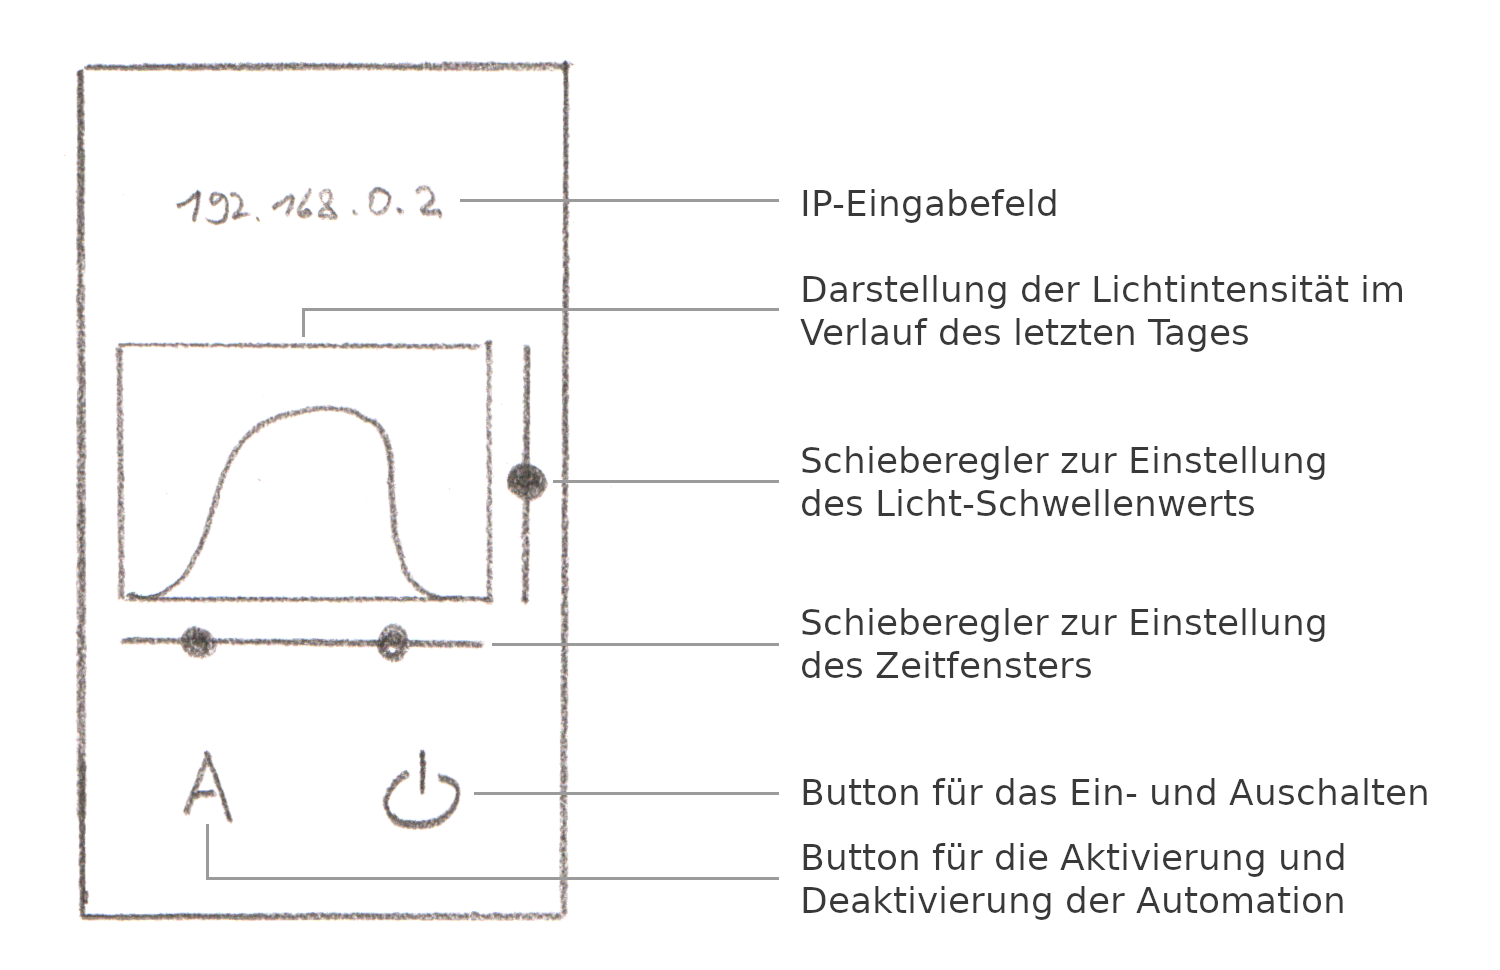
\includegraphics[width=0.95\textwidth]{resources/own_content/App_Design_Description}
	\caption{User Interface Entwurf \cite{LeIn}}
	\label{img:design_interface}
\end{figure}



 \clearpage
\chapter{Implementierung}

\section{Hardware}

\subsection{Implementierung Beleuchtungshardware}
Das Design von Matthew Perks wurde für die Umsetzung der Beleuchtung modifiziert. Die Lichtquelle stellt in diesem Projekt eine 100w LED mit einem CRI-Index von 95 und einem Kelvinwert von 5600 dar. Das abgegebene Licht entspricht in der Helligkeit, Qualität und Farbe in etwa Morgenlicht. Diese LED wird von einem 300w starken, gebrauchten CPU Kühler bei einer Arbeitstemperatur von unter 60 gehalten. Dieser überdimensionierte Kühler wurde aus dem Grund gewählt, dass der verbaute Lüfter sich bei einer relativ geringen Last nur langsam drehen muss und damit leise operiert. Die LED mit Kühler wurde anstelle der Antenne an eine gebrauchte Satellitenschüssel montiert. Die Satellitenschüssel wurde mit Spiegelfolie ausgelegt und wurde damit zu einem Parabolspiegel konvertiert. Mit ihm werden die Strahlen der LED parallel ausgerichtet. Da die LED einen Abstrahlwinkel von fast 180 Grad besitzt, wurde zudem ein Reflektor zur Fokussierung der Strahlen auf den Spiegel verbaut, um nicht zu viel Strahlungsverluste zu haben. Die Stromversorgung wird durch ein 36v AC-DC Netzteil gewährleistet. Damit die LED ihre benötigten 38v erhält, wird der Strom durch ein Step-UP-Modul auf die entsprechende Spannung angehoben. Auch für die Steuerung der Lüfter, die LED und Netzteil kühlen, musste der Strom gewandelt werden. Hierfür wurde ein Step-Down Modul verwendet, welches die Spannung auf 5v herunter wandelt. Dies resultiert in eine konstant niedrige Drehzahl der Lüfter.

\subsection{Implementierung Steuerungshardware}

Um die Beleuchtungshardware drahtlos ansteuern zu können, benötigt es weitere Hardware. Die Wahl eines entsprechenden Mikrocontroller fiel, durch Raten von Pro. Dr. A. Huhn, auf den esp32. Dieser bringt unter anderem die Möglichkeit der Kommunikation via Wifi, die Unterstützung von Mikropyhton, einfache Programmierbarkeit über ein USB-Interface und diverse Optionen zur Stromversorgung mit sich. Nicht zuletzt durch seinen niedrigen Preis stellt er durch seinen Funktionsreichtum eine ideale Option für diese Projekt dar. Die Stromversorgung des Mikrocontroller kann glücklicherweise von dem selben Step-Down Modul übernommen werden, das auch die Lüfter betreibt. Dies ist möglich, da das gewählte ESP-Bord durch die Implementierung eines USB-Interfaces mit internem Step-Down Wandler, nicht nur eine Betriebsspannung von 3,3v, sondern auch 5v-10v unterstützt. Intern nutzt dieses Board jedoch 3,3 für die Signalweitergabe und um seine I/O-Pins zu betreiben. Dies ist viel zu gering um die genutzte LED zu betreiben. Aus diesem Grund muss eine weitere Komponente für die Steuerung der Lampe genutzt werden. Hierzu wird ein Relais verwendet, das mit einer Spannung von 3,3v angesteuert werden kann und 300w Leistung verträgt. Ein weiteres wird für die Steuerung der Lüfter verwendet. Zuletzt braucht der esp32 noch die Möglichkeit die Lichtintensität zu messen. Hierfür wurde ein Lichtsensor verwendet, der über ein I2C-Interface kommuniziert und die Intensität in LUX misst.

\section{Software}
Die Implementierung des Konzepts wurde zunächst anhand von atomaren Prototypen iterativ vorangetrieben. Später flossen diese Erfahrung im Endprodukt zusammen. Dabei spaltet sich dieser Schritt in die Android- und die Micropython-Entwicklung auf. Der Arbeitstitel für die Android-App ist \glqq SunControl\grqq{} und für den Python-Code \glqq SunNode\grqq{}.


\subsection{Implementierung SunControl}
Die Android-Applikation ist sehr simpel gehalten. Die Anzeige wird von einer einzelnen Aktivität übernommen. Diese implementiert ein Interface namens \glqq Displayable\grqq{}, das zur Anzeige aller relevanten Parameter genutzt werden kann. Der \glqq CommunicationHandler\grqq{} wird für die Verarbeitung von ein- und ausgehender Kommunikation genutzt.

Eine Verbindung wird nach Bedarf vom CommunicationHandler über ein \glqq SimpleConnection\grqq{}-Object gestarted. Diesem werden alle nötigen Parameter für eine Anfrage, wie die Nachricht, IP und Port der SunNode und ein observierbarer String, übergeben. Über letzteren wird via dem Observer-Pattern die Antwort der SunNode behandelt. Jedes SimpleConnectionObject eröffnet für die Anfrage einen neuen Thread und terminiert nach Erhalten der Antwort wieder. Damit nicht jedes mal die IP der SunNode neu eingegeben werden muss, wird diese vom CommunicationHandler über den \glqq PreferenceManger\grqq{} des Android-Frameworks persistent gespeichert und bei einem Neustart wiederhergestellt.

Um den Graphen darzustellen wurde eine Bibliothek namens \glqq GraphView\grqq{} verwendet. Diese verlangt das Setzen von Maximalwerten auf der X- und Y-Achse. Um Messpunkte anzeigen zu können, müssen sie als \glqq LineGraphSeries\grqq{} vorliegen. Jeder \glqq DataPoint\grqq{} in dieser Serie verfügt über einen x- und z-Wert. Die Funktion \glqq displayGraph(List<Doubel> list)\grqq{} nimmt die Konvertierung von einem eindimensionalen Array zu solchen Werten vor und teilt die Übergebenen Werte chronologisch auf der X-Achse auf.

Damit die Zeitpunkte für das Ein- und Ausschalten, sowie das kritische Lichtlevel eingestellt werden können, wurden Slider verwendet. Google biete mit \glqq Material Components\grqq{} eine eigene Implementierung dieser an. Um auf Veränderungen ihrer Position reagieren zu können, muss das OnSliderTouchListener Interface implementiert werden. \glqq OnTimeSliderTouchListener\grqq{} und \glqq OnLightSliderTouchListener\grqq{} stellen die jeweiligen konkreten Implementierungen dafür da. Um dem Nutzer beim Verstellen der Zeit den richtigen Zeitpunkt in Form eines Labels anzeigen zu können, wurde zudem ein \glqq TimelabelFormatter\grqq{} auf Basis des \glqq LabelFormatter\grqq{} Interfaces implementiert. Diese Implementierung konvertiert in ihrer einzigen Methode die Dezimalwerte des Zahlenstrahles in eine konventionelle Uhrzeit um.

\subsection{Implementierung SunNode}
Die SunNode besteht aus fünf grundlegenden Komponenten. Standardmäßig existieren in dem Verzeichnis des esp32 schon \glqq boot\grqq{} und \glqq main\grqq{} wobei main bei Stromzufuhr automatisch gestartet wird. Aus diesem Grund werden hier die fünf Komponenten nach ihren Abhängigkeiten chronologisch initialisiert:

\begin{lstlisting}[caption={Initialisierungen in main}, captionpos=b, label={lst:tf_graph_save}]
controller = Controller()
lightsensor = LightSensor()
protocol_machine = ProtocolMachine(controller, lightsensor)
networking = Networking(protocol_machine)
scheduler = Scheduler(controller, lightsensor)
\end{lstlisting}

Wie im vorhergehenden Codeausschnitt zu sehen, haben \glqq networking\grqq{} und \glqq scheduler\grqq{} beide direkt oder indirect zugriff auf \glqq controller\grqq{} und \glqq light\_sensor\grqq{}. Scheduler und networking starten beide Threads von denen nach der Initialisierung der Klassen alle weiteren Methodenaufrufe ausgehen.

Networking ist der Einstiegspunkt für Kommunikation. Bei der Initialisierung stellt er zunächst, anhand der SSID des Netzwerk und des Passworts, die in entsprechenden Dateien gespeichert sind, eine Netzwerkverbindung her. Zudem synchronisiert er die interne Uhr via NTP. Danach hört er auf Port 50000 auf eine Anfrage. Wenn er eine Anfrage bekommt, leitet er sie an protocol\_machine weiter. Diese verarbeitet die Anfrage und gibt eine Antwort zurück. Nachdem diese Antwort zurück an dem Anfragenden geschickt wurde, wird die Verbindung getrennt und der Port kehrt wieder in den wartenden Zustand zurück.

Die protocol\_machine hat zwei grundlegende Aufgaben. Zum einen interpretiert sie die eingehende Anfrage und entscheidet, welche Aktion der controller ausführen soll. Zum anderen gibt sie in jedem Fall eine Antwort zurück. Diese besteht aus allen relevanten Informationen, die zur Anzeige des Status der SunNode gebraucht werden. Denn nach jeder Anfrage könnten sich diese Informationen durch neue Konfigurationen geändert haben und werden deswegen für die Synchronisation der Anzeigen der SunControl benötigt. In jedem Fall werden sowohl Daten von dem controller, als auch dem light\_sensor angefordert.

Light\_sensor stellt die Schnittstelle zum Lichtsensor dar und sammelt Daten zum aktuellen und vorhergehenden Tag. Dazu zählen alle gesammelten Lichtmesspunkte in diesen Zeiträumen und der insgesamte Höchstwert. Der Höchstwert ist deswegen wichtig, da anhand von ihm die y-Achse des Graphen der SunControll skaliert wird. Wenn die Daten des letzten Tages angefordert werden, jedoch noch kein kompletter Tag seit dem ersten Messpunkt vergangen ist, werden die bisher gesammelten Messpunkte zurück gegeben. Dies geschieht, um trotz unvollständiger Informationen, dem Nutzer einen Orientierungspunkt für Einstellungen bieten zu können.

Der Controller steuert das physikalische Licht. Er stellt zudem die Datenbasis für alle notwendigen Parameter, die bei Anfragen oder einer Änderung des Lichtlevels für die Bewertung der Situation nötig sind. Alle Parameter, die über SunControll gesetzt werden, sind hier gespeichert. Zudem wird der letzte Messpunkt des light\_sensor hier hinterlegt, um gegebenenfalls außerhalb der Messintervalle auf ihn zugreifen zu können.

Die letzte Komponente ist scheduler. Sie ist Taktgeber zur Messung und löst alle autonomen Events aus. Alle 15 Minuten lässt sie den light\_sensor eine Messung ausführen und gibt das Ergebnis an den controller weiter, der je nach Wert und Einstellungen entsprechend reagiert. Das Intervall von 15 Minuten wurde deswegen gewählt, da es noch eine realistisch feine Abstufung zur Einstellung von Weckzeiten darstellt. Feinere Werte haben in Testläufen dazu geführt, dass der interne Speicher des Mikrocontrollers nicht mehr für die Speicherung aller Werte des Tages ausgereicht hat und das Programm deswegen abstürzte. 15 Minuten ist ein Kompromiss zwischen ausreichender Einstellungsgranularität und dieser Hardwarelimitierung. Eine tiefere Ausführung dazu folgt im nächsten Kapitel. 






 \clearpage
\chapter{Test}

\section{SunNode Test}
Um Erfahrungen mit Micropyhton zu sammeln und die zu verwendenden Konzepte aus zu testen, wurden schon vor der Entwicklungsphase atomare Tests durchgeführt. Dabei wurde die Netzwerkverbindung als Server sowie Client, die Messung des Lichtlevels über den Sensor, sowie die Ansteuerung der Relais ausgetestet. Später sollten Unit-Tests hinzugefügt werden. Dieser Plan wurde jedoch durch die fehlenden Standardmöglichkeiten zum Mocken von Micropython-Klasen stark erschwert. Auch nach langer Recherche wurde keine passende Alternative gefunden, weswegen auf manuelle Integrationstest gesetzt wurde. Zwar wäre eine eigene Implementation von Mock-Klassen grundsätzlich machbar, jedoch würde dies den Rahmen dieser Arbeit sprengen.
Bei dieser Art des Testens wurden  Speicherlimitation des Esps und oder architektonische Probleme erkenntlich. Denn durch die Speicherung von primitiven Zahlen wie Integers oder Floats als Objekte, benötigt Micropyhton ca. dreimal so viel Platz, als für den Wert alleine nötig wäre. Dies stellt eine sehr ineffiziente Art der Speicherung auf einer so stark limitierten Plattform da. Eine Möglichkeit dieses Problem zu umgehen wäre den Speicher an sich zu erweitern. Zu diesem Zweck gibt es Module für die Anbindung einer SD-Karte, die mit dem Esp kompatibel sind. Da für den vorgesehenen Einsatzzweck 15 Minutenintervalle als ausreichend angesehen wurden, konnte jedoch eine niedrigere Messfrequenz die Speicherlimitierung umgehen.

\section{SunControl Test}
SunControl hat einen sehr geringen Funktionsumfang. Da es fast ausschließlich für die Visualisierung von Daten der SunNode zuständig ist, macht es wenig Sinn viele Unit-Tests zu schreiben, da diese fast ausschließlich die Funktion der Getter- und Setter-Methoden des Android-Frameworks testen würden und ob sie in der richtigen Reihenfolge aufgerufen wurden. Eines Ausnahme bildet die TimeLabelFormatter-Klasse. Sie ist für die Umwandlung von geschriebener Zeit in eine Dezimalzahl und zurück zuständig. \clearpage
\chapter{Evaluation}
\label{SunNode}
Die SunNode erfüllt ihren vorgesehenen Zweck größtenteils. Das Licht schaltet sich bei den eingestellten Uhrzeiten und entsprechenden Beleuchtungsumständen an und auch wieder aus. Die Kommunikation mit SunControl verläuft zügig und gibt bei Veränderungen zeitnah Feedback. Dabei bleibt das Programm stabil und verhält sich vorhersehbar.
Es besteht jedoch ernsthaftes Verbesserungspotential, das über einen höheren Featureumfang hinausgeht. Denn durch die Verwendung von NTP schaltet der esp32 nicht automatisch zwischen Winter und Sommerzeit um. Dieser Umstand ist nicht durch Bordmittel von Mircopython zu ändern und benötigt eine eigene Implementierung. Da  Python diese Funktion mitbringt und die Nutzung von Zeit in Programmcodes nicht selten vorkommen sollte, stellt sich die Frage, wieso Micropython dies nicht anbietet. Mit dem momentanen Stand der Dinge hinkt die Uhr der SunNode während der Winterzeit eine Stunde zurück.

\section{SunControl}
Auch die SunControl erfüllt ihren vorgesehenen Zweck größtenteils. So zeigt sie relevante Informationen für den Nutzer an und reagiert zügig und vorhersehbar auf Eingaben. Das Nutzerinterface entspricht dabei dem ursprünglichem Konzept vollkommen. Bei der Anzeige kann jedoch ein Problem zu Tage treten: Die Anzeige wird nur einmal beim Öffnen der Applikation aktualisiert und nach jeder Interaktion mit den Einstellungsmöglichkeiten. Wenn sich das Licht während einer interaktionslosen Phase automatisch ausschaltet, oder ein anderer Nutzer Änderungen vornimmt, wird dies nicht in dem Nutzerinterface widergespiegelt. Dies liegt an der grundlegenden Kommunikationsweise zwischen SunControl und SunNode, die der SunNode nicht die Möglichkeit gibt, ihre Observer über Änderungen zu informieren. Dies klingt in der Theorie problematisch, sollte im alltäglichen Gebrauch jedoch kaum auffallen. Denn an einem typischen Tag sollte das Licht sich vier mal an- oder ausschalten, wodurch es nicht sehr wahrscheinlich ist, das dies bei einer vermutlich kurzen und seltenen Interaktion mit der Applikation, vorkommt. Auch Mehrnutzerbetrieb sollte so gut wie nicht vorkommen, da es sich um eine einzelne Beleuchtung handelt.

\section{Hardware}
Die Hardware erfüllt genau den Zweck ihres Konzepts. Das abgegebene Licht erinnert an Morgensonne und wurde von den bisherigen Nutzern als motivations- und konzentrations-steigernd empfunden.
Die Implementierung zeigt jedoch Schwachstellen am ursprünglichem Konzept. Denn wenn die Sonnen von Wolken verdeckt wird und das Lichtschaltlevel zwischen der Helligkeit bei freiem Himmel und verdecktem Himmel gesetzt wurde, kann es zum wiederkehrendem Ein- und Ausschalten des Lichtes kommen. 
Eine Modifikation des ursprünglichem Hardware-Designs könnte hier Abhilfe schaffen. So könnte ein Dimmer in Echtzeit die Helligkeit anpassen, ohne Flackern zu verursachen oder durch extreme Helligkeitswechsel zu irritieren.
 \clearpage
\chapter{Fazit}

\section{Zusammenfassung}
Eine Beleuchtung zu designen, die Sonnenlicht realistisch Nachahmen kann, ist keine kleine Aufgabe. Es gibt viele Produkte, die Elemente davon simulieren können. Jedoch gibt es trotz verschiedener Konzepte bis jetzt keine Produkte auf dem Markt, das so viele Elemente davon vereint. Dies ist eine bemerkenswerte Marktlücke, den viele Bereiche des Lebens könnten von einem solchen Produkt profitieren. Nachtschichten könnten sich erfrischender anfühlen, Wintermonate sich nicht so lange anfühlen und sogar komplett neue Wohnkonzepte erschlossen werden.

\section{Kritischer Rückblick}
Diese Projektarbeit hat gezeigt, dass bereits alle Technologien für eine realistische Simulation von Sonnenlicht existieren. Es ist nur eine Frage der Implementierung, diese Stücke zu einem großen Ganzen zu vereinen. Ob tatsächlich jemand ein so helles Licht in seinem Wohnzimmer braucht, ist zu hinterfragen. Viele weitere Eigenschaften sind aber durchaus wünschenswert auch wenn nicht alle in diesem Projekt realisiert wurden. Der wortwörtlich größte Schwachpunkt dieser Implementierung ist die physikalischen Dimensionen der benötigen Hardware. Wenn man parallele ausgerichtetes Licht erzeugen möchte, braucht man eine Vorrichtung mit der selben Höhe und Breite, die der Strahl besitzen soll. In Verbindung mit einem Parabolspiegel kommt zudem eine proportional große Tiefe hinzu. Dieses Projekt verbraucht damit einen knappen Kubikmeter an Platz. Zudem ist für einen realistischen Effekt ratsam, das Licht wie ein (Dach)-Fenster zu platzieren. Dies stellt einen guten Grund für die geringe Adaption dieses Ansatzes in kommerziellen Produkten dar. 

\section{Ausblick}
Innovationen können die Limitationen dieser Lösung in Zukunft hoffentlich überkommen. Neue Beleuchtungskonzepte sind gefragter den je, was nicht zuletzt durch IKEAs hauseigene vernetzte Beleuchtungssystem erkenntlich ist. Bis sich kommerzielle Produkte weiterentwickelt haben, bleibt leider nur der Weg des Eigenbaus. \clearpage

\pagenumbering{Roman}
% List of Figures
\listoffigures \clearpage
% Source Code Content
\lstlistoflistings \clearpage

\printindex \clearpage

\defbibfilter{scientific}{
	type=article or
	type=inbook or
	type=book or
	type=unpublished or
	type=inproceedings or
	type=incollection or
	type=manual or
	type=phdthesis
}

\printbibliography[heading=bibintoc, keyword={online}, title={Onlinereferenzen}]\clearpage
\printbibliography[heading=bibintoc, keyword={image}, title={Bildreferenzen}]\clearpage

% Eigenständigkeitserklärung (CHOOSE ONE)
%\input{erklaerungen/Eigenstaendigkeitserklaerung_bachelorthesis} % FOR BACHELORTHESIS
%\input{erklaerungen/Eigenstaendigkeitserklaerung_masterthesis} % FOR MASTERTHESIS
\addchap{Eigenständigkeitserklärung}

Hiermit versichere ich, dass ich die vorliegende Arbeit selbstständig und nur unter Verwendung der angegebenen Quellen und Hilfsmittel verfasst habe. Die Arbeit wurde bisher in gleicher oder ähnlicher Form keiner anderen Prüfungsbehörde vorgelegt.

\vskip 1cm

Berlin, den 26.03.2021


\includegraphics[height=5\baselineskip]{resources/own_content/Leon-Unterschrift}

Leon Enzenberger
 % FOR RESEARCH PROJECT

\end{document}
